%%%%%%%%%%%%%%%%%%%%%%%%%%%%%%%%%%%%%%%%%
% Beamer Presentation
% LaTeX Template
% Version 1.0 (10/11/12)
%
% This template has been downloaded from:
% http://www.LaTeXTemplates.com
%
% License:
% CC BY-NC-SA 3.0 (http://creativecommons.org/licenses/by-nc-sa/3.0/)
%
%%%%%%%%%%%%%%%%%%%%%%%%%%%%%%%%%%%%%%%%%

%----------------------------------------------------------------------------------------
%	PACKAGES AND THEMES
%----------------------------------------------------------------------------------------

\documentclass{beamer}

\mode<presentation> {

% The Beamer class comes with a number of default slide themes
% which change the colors and layouts of slides. Below this is a list
% of all the themes, uncomment each in turn to see what they look like.

%\usetheme{default}
%\usetheme{AnnArbor}
%\usetheme{Antibes}
%\usetheme{Bergen}
%\usetheme{Berkeley}
%\usetheme{Berlin}
%\usetheme{Boadilla}
%\usetheme{CambridgeUS}
%\usetheme{Copenhagen}
%\usetheme{Darmstadt}
%\usetheme{Dresden}
%\usetheme{Frankfurt}
%\usetheme{Goettingen}
%\usetheme{Hannover}
%\usetheme{Ilmenau}
%\usetheme{JuanLesPins}
%\usetheme{Luebeck}
\usetheme{Madrid}
%\usetheme{Malmoe}
%\usetheme{Marburg}
%\usetheme{Montpellier}
%\usetheme{PaloAlto}
%\usetheme{Pittsburgh}
%\usetheme{Rochester}
%\usetheme{Singapore}
%\usetheme{Szeged}
%\usetheme{Warsaw}

% As well as themes, the Beamer class has a number of color themes
% for any slide theme. Uncomment each of these in turn to see how it
% changes the colors of your current slide theme.

%\usecolortheme{albatross}
%\usecolortheme{beaver}
%\usecolortheme{beetle}
%\usecolortheme{crane}
%\usecolortheme{dolphin}
%\usecolortheme{dove}
%\usecolortheme{fly}
%\usecolortheme{lily}
%\usecolortheme{orchid}
%\usecolortheme{rose}
%\usecolortheme{seagull}
%\usecolortheme{seahorse}
%\usecolortheme{whale}
%\usecolortheme{wolverine}

%\setbeamertemplate{footline} % To remove the footer line in all slides uncomment this line
%\setbeamertemplate{footline}[page number] % To replace the footer line in all slides with a simple slide count uncomment this line

%\setbeamertemplate{navigation symbols}{} % To remove the navigation symbols from the bottom of all slides uncomment this line
}

\usepackage{graphicx} % Allows including images
\usepackage{booktabs} % Allows the use of \toprule, \midrule and \bottomrule in tables

\usepackage[UTF8]{ctex}
\usepackage{verbatim}
\usepackage[backend=bibtex,style=authoryear,natbib=true,backref=true]{biblatex}
\addbibresource{../ref/ref.bib} % The filename of the bibliography
\usepackage[]{algorithm2e}
\renewcommand{\algorithmcfname}{算法}
\usepackage{verbatim}

\AtBeginSection[]
{
\begin{frame}{目录}
\tableofcontents[currentsection]
\end{frame}
}

\AtBeginSubsection[]  %该函数在每到一个subsection是就显示整篇文章的目录
{
\begin{frame}{目录}
\tableofcontents[currentsection,currentsubsection]
\end{frame}
}

%----------------------------------------------------------------------------------------
%	TITLE PAGE
%----------------------------------------------------------------------------------------

\title[L1-TWSVM]{L1-TWSVM} % The short title appears at the bottom of every slide, the full title is only on the title page

\author{闫茹钰, 喻望, 张芙作, 郑洁, 朱榕平} % Your name
\institute % Your institution as it will appear on the bottom of every slide, may be shorthand to save space
{
自动化系 \\ % Your institution for the title page
}
\date{\today} % Date, can be changed to a custom date

\begin{document}

\begin{frame}
\titlepage % Print the title page as the first slide
\end{frame}

\begin{frame}
\frametitle{目录} % Table of contents slide, comment this block out to remove it
\tableofcontents % Throughout your presentation, if you choose to use \section{} and \subsection{} commands, these will automatically be printed on this slide as an overview of your presentation
\end{frame}

%----------------------------------------------------------------------------------------
%	PRESENTATION SLIDES
%----------------------------------------------------------------------------------------

%------------------------------------------------
\section{TWSVM} % Sections can be created in order to organize your presentation into discrete blocks, all sections and subsections are automatically printed in the table of contents as an overview of the talk
%------------------------------------------------

\begin{frame}
\frametitle{TWSVM}
TWSVM (孪生支持向量机) 是 Jayadeva 等人于2007年提出的一种改进的双分界面支持向量机,用于解决二分类问题。
\begin{columns}
\column{0.5\textwidth}
\small{
\begin{align}
\begin{split}
\label{ts1}
\min_{\mathbf{w}_1,b_1} \; & \frac{1}{2}\|\mathbf{Aw}_1+\mathbf{e}_1b_1\|_2^2+c_1\mathbf{e}_2^T\mathbf{q}_1 \\
s.t.\; & -(\mathbf{Bw}_1+\mathbf{e}_2b_1)+\mathbf{q}_1 \geq \mathbf{e}_2 \\
&\mathbf{q}_1\geq 0
\end{split}
\\
\begin{split}
\label{ts2}
\min_{\mathbf{w}_2,b_2} \; & \frac{1}{2}\|\mathbf{Bw}_2+\mathbf{e}_2b_2\|_2^2+c_2\mathbf{e}_1^T\mathbf{q}_2 \\
s.t. \; & (\mathbf{Aw}_2+\mathbf{e}_1b_2)+\mathbf{q}_2\geq \mathbf{e}_1 \\
&\mathbf{q}_2\geq 0
\end{split}
\end{align}
}

\column{0.5\textwidth}<2->
\begin{figure}[ht]
\centering
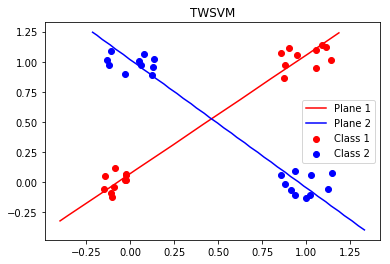
\includegraphics[width=0.9\textwidth]{../img/TWSVM-img.png}
\label{twsvm1}
\end{figure}
\end{columns}
\end{frame}

%------------------------------------------------

\begin{frame}
\frametitle{TWSVM 对偶问题}
\begin{align}
\begin{split}
\max\limits_{\pmb{\alpha}} \; & \mathbf{e}_2^T \pmb{\alpha}-\frac{1}{2}\pmb{\alpha}^T\mathbf{G}(\mathbf{H}^T\mathbf{H})^{-1}\mathbf{G}^T\pmb{\alpha} \\
s.t. \; & 0 \leq \pmb{\alpha}\leq c_1 \mathbf{e}_2
\end{split}
\\
\begin{split}
\max\limits_{\pmb{\beta}} \; & \mathbf{e}_1^T \pmb{\beta}-\frac{1}{2}\pmb{\beta}^T\mathbf{H}(\mathbf{G}^T\mathbf{G})^{-1}\mathbf{H}^T\pmb{\beta} \\
s.t. \; & 0 \leq \pmb{\beta} \leq c_2\mathbf{e}_1
\end{split}
\end{align}
\end{frame}

%------------------------------------------------
\section{L1-TWSVM}
\begin{frame}
\frametitle{L1-TWSVM 优化问题}
TWSVM 有良好的分类性能,已成为数据分类研究的热点。但 TWSVM 使用对离群值较为敏感的 L2 范数来度量距离,导致异常观测点可能会对其结果有较大影响。由于 L1 范数是 L2 范数距离的鲁棒替代,\parencite{yan2018efficient} 提出基于 L1 范数的鲁棒分类器。
\begin{align}
\begin{split}
\label{ts3}
    \min\limits_{\mathbf{w}_1,b_1} \;& \frac{1}{2}||\mathbf{Aw}_1+\mathbf{e}_1b_1||_1+c_1\mathbf{e}_2^T\mathbf{q}_1 \\
    s.t.\;& -(\mathbf{Bw}_1+\mathbf{e}_2b_1)+\mathbf{q}_1 \geq \mathbf{e}_2,\mathbf{q}_1\geq 0
\end{split}
\\
\begin{split}
\label{ts4}
    \min\limits_{\mathbf{w}_2,b_2} \;& \frac{1}{2}||\mathbf{Bw}_2+\mathbf{e}_2b_2||_1+c_2\mathbf{e}_1^T\mathbf{q}_2 \\
    s.t. \; &(\mathbf{Aw}_2+\mathbf{e}_1b_2)+\mathbf{q}_2\geq \mathbf{e}_1, \mathbf{q}_2\geq 0
\end{split} 
\end{align}
\end{frame}

%------------------------------------------------

\begin{frame}
\frametitle{L1-TWSVM 求解思路}
原问题可改写为
\begin{align}
\begin{split}
\label{ts5}
    \min\limits_{\mathbf{w}_1,b_1} \;& \frac{1}{2}(\sum_{i=1}^{m_1}\frac{(\mathbf{a}_i^T\mathbf{w}_1+e_1^ib_1)^2}{d_i})+c_1\mathbf{e}_2^T\mathbf{q}_1  \\
    s.t.\;& -(\mathbf{Bw}_1+\mathbf{e}_2b_1)+\mathbf{q}_1 \geq \mathbf{e}_2,\mathbf{q}_1\geq 0
\end{split}
\end{align}
其中 $d_i=|\mathbf{a}_i^T\mathbf{w}_1+e_1^ib_1|\ne 0$。令 $\mathbf{D}_1=diag(1/d_{11},1/d_{12},\ldots,1/d_{1m_1})$,则问题即为
\begin{align}
\begin{split}
\label{ts8}
    \min\limits_{\mathbf{z}_1} \;& \frac{1}{2}\mathbf{z}_1^T\mathbf{H}^T\mathbf{D}_1\mathbf{Hz}_1+c_1\mathbf{e}_2^T\mathbf{q}_1 \\
    s.t.\;& -(\mathbf{Gz}_1+\mathbf{q}_1) \geq \mathbf{e}_2,\mathbf{q}_1\geq 0
\end{split}
\end{align}
\end{frame}

\begin{frame}
\frametitle{L1-TWSVM 算法}
\begin{algorithm}[H]
 \textbf{Input}: $A \in \mathbb{R}^{m_1 \times n}$ and $B \in \mathbb{R}^{m_2 \times n}$\;
 Construct the matrices $H = (A\; e_1)$ and $G = (B\; e_2)$\;
 Set $p = 0$. Initialize $z^p$, a standard solution of TWSVM\;
 \While{not converge}{
  Compute $D_1^p$\;
  Compute $z_1^{(p+1)}$ by solving
  \begin{equation}
  \label{algo1}
  z_1^{(p+1)} = \mathop{\arg\min}_{z_1} \frac{1}{2}z_1^TH^TD_1^pHz_1 + c_1e_2^Tq_1,\;s.t.\,-Gz_1+q_1\geq e_2,\,q_1\geq 0
  \end{equation}
  p=p+1;
 }
 \textbf{Output}: The learned solution of $z_1$.
\end{algorithm}
\end{frame}

%------------------------------------------------

\section{L1-TWSVM 收敛性证明}

\begin{frame}
\frametitle{L1-TWSVM 收敛性证明}
\begin{lemma}
对任意非零向量 $\mathbf{u},\mathbf{u}^p\in\mathbb{R}^1$,有以下不等式:
\begin{equation}
\|\mathbf{u}\|_{1}-\frac{\|\mathbf{u}\|^{2}_{1}}{2\|\mathbf{u}^p\|_{1}}\le
\|\mathbf{u}^p\|_{1}-\frac{\|\mathbf{u}^p\|^{2}_{1}}{2\|\mathbf{u}^p\|_{1}}
\label{yw1}
\end{equation}
\end{lemma}

\begin{proof}
\begin{equation}
\begin{aligned}
&(\sqrt{\mathbf{v}}-\sqrt{\mathbf{v^p}})^2\ge0
\Rightarrow\mathbf{v}-2\sqrt{\mathbf{vv}^p}+\mathbf{v}^p\ge0\\
&\Rightarrow\sqrt{\mathbf{v}}-\frac{\mathbf{v}}{2\sqrt{\mathbf{v}^p}}\le
\frac{\sqrt{\mathbf{v}^p}}{2}
\Rightarrow\sqrt{\mathbf{v}}-\frac{\mathbf{v}}{2\sqrt{\mathbf{v}^p}}\le
\sqrt{\mathbf{v}^p}-\frac{\mathbf{v}^p}{2\sqrt{\mathbf{v}^p}}
\end{aligned}
\label{yw2}
\end{equation}
\end{proof}
\end{frame}

\begin{frame}[allowframebreaks]
\frametitle{L1-TWSVM 收敛性证明}
\begin{theorem}
算法1在每步迭代中都使问题 \eqref{ts8} 的目标值单调递减。
\end{theorem}

\textbf{【证明】}
首先,用以下等式重写 \eqref{algo1} 中的问题:
\begin{equation}
\mathbf{z}^{(p+1)}_{1}=\mathop{\arg\min}_{\mathbf{z}_{1}}
\frac{1}{2}\mathbf{z}^{T}_{1}\mathbf{H}^{T}\mathbf{D}^{T}_{1}\mathbf{H}\mathbf{z}_{1}+
c_{1}\mathbf{e}^{T}_{2}\mathop{\max}(0,\mathbf{e}_{2}+\mathbf{Gz}_{1})
\label{yw3}
\end{equation}
即:
\begin{equation}
\mathbf{z}^{(p+1)}_{1}=\mathop{\arg\min}_{\mathbf{z}_{1}}
\frac{1}{2}(\mathbf{Hz}_{1})^{T}\mathbf{D}^{p}_{1}\mathbf{Hz}_{1}+
c_{1}\mathbf{e}^{T}_{2}\mathop{\max}(0,\mathbf{e}_{2}+\mathbf{Gz}_{1})
\label{yw4}
\end{equation}
因此,在第 $(p+1)$ 步迭代中,有
\begin{equation}
\begin{aligned}
&\frac{1}{2}(\mathbf{Hz}^{(p+1)}_{1})^{T}\mathbf{D}^{p}_{1}(\mathbf{Hz}^{(p+1)}_{1})+
c_{1}\mathbf{e}^{T}_{2}\mathop{\max}(0,\mathbf{e}_{2}+\mathbf{Gz}^{(p+1)}_{1})\\
&\le\frac{1}{2}(\mathbf{Hz}^{p}_{1})^{T}\mathbf{D}^{p}_{1}(\mathbf{Hz}^{p}_{1})+
c_{1}\mathbf{e}^{T}_{2}\mathop{\max}(0,\mathbf{e}_{2}+\mathbf{Gz}^{p}_{1})
\end{aligned}
\label{yw5}
\end{equation}
将式 \eqref{yw1} 中的 $\mathbf{u}$ 和 $\mathbf{u}^p$ 替换为 $\mathbf{Hz}^{(p+1)}_{1}$ 和 $\mathbf{Hz}^{p}_{1}$,可以得到:
\begin{equation}
\|\mathbf{Hz}^{(p+1)}_{1}\|_{1}-\frac{\|\mathbf{Hz}^{(p+1)}_{1}\|^{2}_{1}}{2\|\mathbf{Hz}^{p}_{1}\|_{1}}\le
\|\mathbf{Hz}^{p}_{1}\|_{1}-\frac{\|\mathbf{Hz}^{p}_{1}\|^{2}_{1}}{2\|\mathbf{Hz}^{p}_{1}\|_{1}}
\label{yw6}
\end{equation}
因此可得如下不等式:
\begin{equation}
\sum^{m_1}_{i=1}(\left|\mathbf{h}^{T}_{i}\mathbf{z}^{(p+1)}_1\right|-
\frac{(\mathbf{h}^{T}_{i}\mathbf{z}^{(p+1)}_1)^2}
{2\left|\mathbf{h}^{T}_{i}\mathbf{z}^{p}_{1}\right|})\le
\sum^{m_1}_{i=1}(\left|\mathbf{h}^{T}_{i}\mathbf{z}^{p}_1\right|-
\frac{(\mathbf{h}^{T}_{i}\mathbf{z}^{p}_1)^2}
{2\left|\mathbf{h}^{T}_{i}\mathbf{z}^{p}_{1}\right|})
\label{yw7}
\end{equation}
该式可被简化为:
\begin{equation}
\begin{aligned}
&\|\mathbf{Hz}^{(p+1)}_{1}\|_{1}-\frac{1}{2}(\mathbf{Hz}^{(p+1)}_{1})^{T}\mathbf{D}^{p}_{1}(\mathbf{Hz}^{(p+1)}_{1})\\
&\le\|\mathbf{Hz}^{p}_{1}\|_{1}-\frac{1}{2}(\mathbf{Hz}^{p}_{1})^{T}\mathbf{D}^{p}_{1}(\mathbf{Hz}^{p}_{1})     \end{aligned}
\label{yw8}
\end{equation}
综合式 \eqref{yw5} 和 \eqref{yw8},可得:
\begin{equation}
\begin{aligned}
&\|\mathbf{Hz}^{(p+1)}_{1}\|_{1}+c_{1}\mathbf{e}^{T}_{2}\mathop{\max}(0,\mathbf{e}_{2}+\mathbf{Gz}^{(p+1)}_{1})\\
&\le\|\mathbf{Hz}^{p}_{1}\|_{1}+c_{1}\mathbf{e}^{T}_{2}\mathop{\max}(0,\mathbf{e}_{2}+\mathbf{Gz}^{p}_{1})
\end{aligned}
\label{yw9}
\end{equation}
因为 \eqref{ts8} 中的问题恒小于零,因此算法1收敛,\eqref{yw9} 中的不等式成立。
\end{frame}

\begin{frame}[allowframebreaks]
\frametitle{L1-TWSVM 收敛性证明}
\begin{theorem}
算法1收敛至问题 \eqref{ts8} 的一个局部最优解。
\end{theorem}

\textbf{【证明】}
问题 \eqref{ts8} 的拉格朗日函数如下:
\begin{equation}
L_{2}(\mathbf{z}_{1},\mathbf{q}_{1})=\frac{1}{2}\|\mathbf{Hz}_{1}\|_{1}+
c_{1}\mathbf{e}^{T}_{2}\mathbf{q}_{1}-\mathbf{\alpha}^{T}(-\mathbf{Gz}_{1}+\mathbf{q}_{1}-\mathbf{e}_{2})
-\mathbf{\beta^{T}q}_{1}
\label{yw10}
\end{equation}
其中,$\mathbf{\alpha}$ 和 $\mathbf{\beta}$ 是拉格朗日乘子向量。通过对其求导并取零,可以得到问题 \eqref{ts8} 的 KKT 条件:
\begin{equation}
\mathbf{H}^{T}\mathbf{D}_{1}\mathbf{Hz}_{1}+\mathbf{G\alpha}=0,
c_{1}\mathbf{e}_{2}-\mathbf{\alpha}-\mathbf{\beta}=0
\label{yw11}
\end{equation}
在算法1的每步迭代中,寻找问题 \eqref{algo1} 中的最优 $\mathbf{z}^{(p+1)}_{1}$ 。
因此,算法1的收敛解满足问题的 KKT 条件。接下来,定义算法1中问题 \eqref{algo1} 的拉格朗日函数如下:
\begin{equation}
L_{3}(\mathbf{z}_{1},\mathbf{q}_{1})=\frac{1}{2}\mathbf{H}^{T}\mathbf{D}_{1}\mathbf{Hz}_{1}+
c_{1}\mathbf{e}^{T}_{2}\mathbf{q}_{1}-\mathbf{\alpha}^{T}(-\mathbf{Gz}_{1}+\mathbf{q}_{1}-\mathbf{e}_{2})
-\mathbf{\beta^{T}q}_{1}
\label{yw12}
\end{equation}
同样对其求导并取零,得到:
\begin{equation}
\mathbf{H}^{T}\mathbf{D}_{1}\mathbf{Hz}_{1}+\mathbf{G\alpha}=0,
c_{1}\mathbf{e}_{2}-\mathbf{\alpha}-\mathbf{\beta}=0
\label{yw13}
\end{equation}
根据算法1中 $\mathbf{D}_{1}$ 的定义,等式 \eqref{yw11} 和 \eqref{yw13} 在算法1收敛时成立。这说明算法1的收敛解 $\mathbf{z}^{(p+1)}_{1}$ 满足问题 \eqref{ts8} 的KKT条件,是问题 \eqref{ts8} 的一个局部最优解。
\end{frame}


\section{数值实验}

\begin{frame}
\frametitle{数值实验}
实验代码采用 Python 编写,调用 cvxpy \parencite{cvxpy} 求解凸优化问题。使用\emph{异或问题}测试 L1-TWSVM 算法的正确性。
\begin{figure}[ht]
\centering
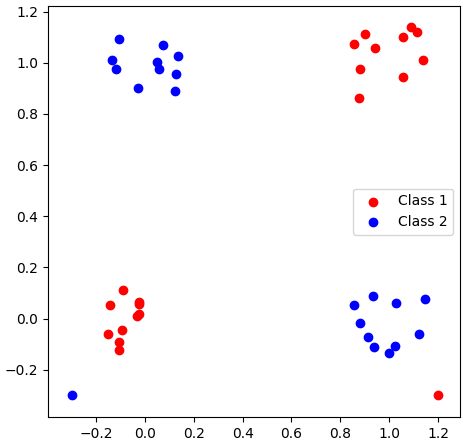
\includegraphics[width=0.4\textwidth]{../img/datas.png}
\caption{数据散点图}
\label{data_points}
\end{figure}
\end{frame}

\begin{frame}
\frametitle{数值实验}
\begin{figure}[ht]
\centering
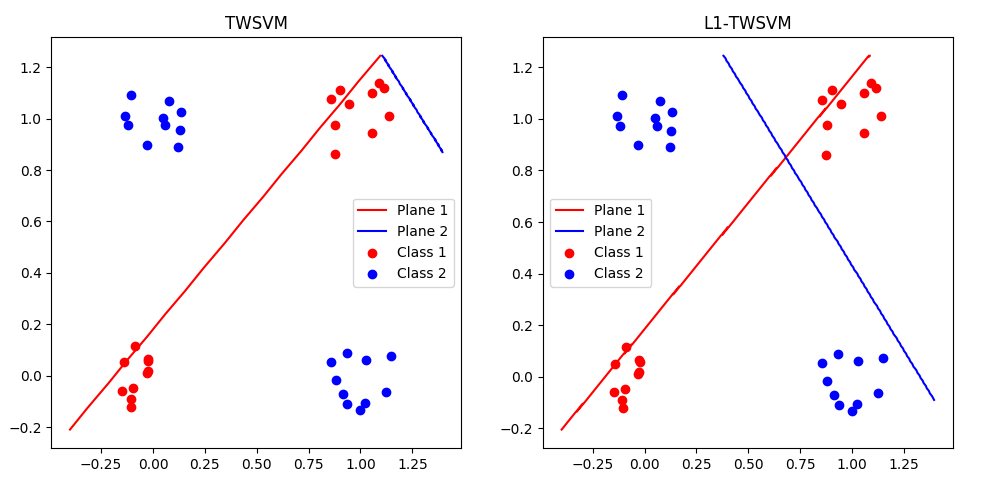
\includegraphics[width=0.8\textwidth]{../img/without_norm_cons.png}
\caption{不带离群点,无参数规范化}
\label{no_out_no_reg}
\end{figure}
\end{frame}

\begin{frame}
\frametitle{数值实验}
\begin{figure}[ht]
\centering
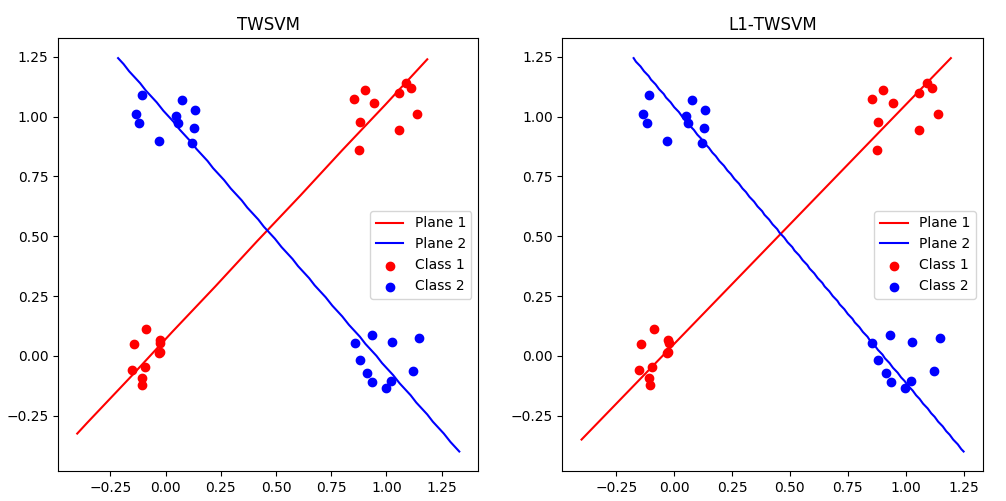
\includegraphics[width=0.8\textwidth]{../img/without_outliers.png}.
\caption{不带离群点,参数规范化}
\label{no_out}
\end{figure}
\end{frame}

\begin{frame}
\frametitle{数值实验}
\begin{figure}[ht]
\centering
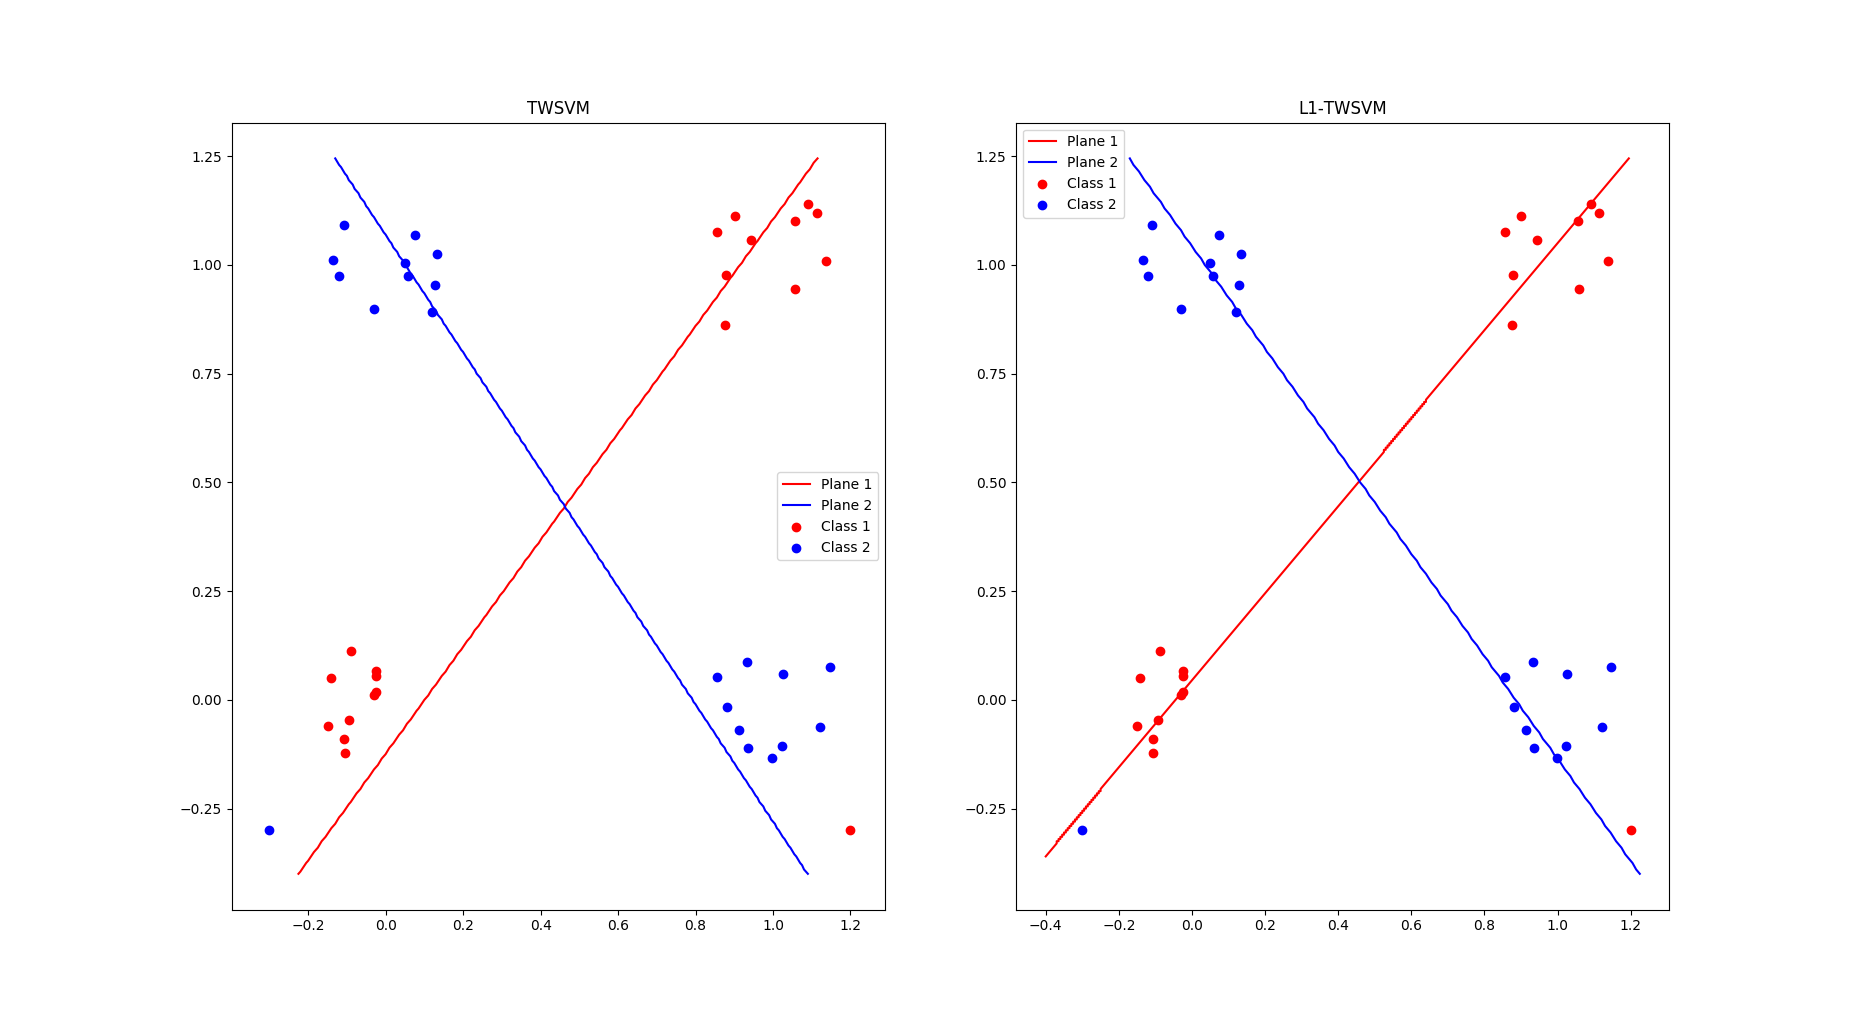
\includegraphics[width=0.8\textwidth]{../img/with_outliers.png}
\caption{带离群点,参数规范化}
\label{outliers}
\end{figure}
\end{frame}

\section{参考文献}
\begin{frame}[allowframebreaks]
\frametitle{参考文献}
\footnotesize{
\printbibliography
}
\end{frame}


\begin{frame}
\Huge{\centerline{谢谢}}
\end{frame}

%----------------------------------------------------------------------------------------

\end{document} 